\chapter{弗里德曼动力学与状态方程}

\lectureoverview{必须将均匀膨胀与局部束缚物理区分开来，也必须将内禀几何与嵌入的形状区分开来。一旦这些区分得以确立，宇宙学原理便将时空度规约化为一个标度因子\(a(t)\)和一个曲率标记\(k\)。爱因斯坦方程的时间-时间分量随即成为弗里德曼能量方程。为求解它，我们仍需要压强与能量密度之间的物质关系。绝热热力学与状态方程\(P=w\rho\)给出\(\rho\propto a^{-3(1+w)}\)，从而将物质、辐射与真空能量统一在一个框架之中。}

\section{确定物理图像的问题}

\subsection{空间能否在视界之前重复？}

一个有限的平直宇宙可以用一个周期性单元来表示。如果该单元小于可观测区域，光便能穿越它，天空中就会包含同一批结构的重复影像。探测这些重复比单纯辨认一个熟悉的星系要困难得多：这些影像来自不同的方向和不同的时期，并且被宇宙演化所改变。尽管如此，周期性拓扑仍具有可观测的后果。

\begin{classroomqa}
\audiencequestion{整个宇宙是否可能小于可观测宇宙？}
\lecturerresponse{周期性认同的环面是自然的候选方案。那样的话，我们观察到的就会是同一物理区域的重复副本，形象地说，就是透过后门看到我们自己。对相应宇宙周期性的搜寻并未产生支持性证据，并且确实对小的基本单元施加了限制。这种可能性在几何上是自洽的，但一个小于已被观测区域的宇宙并未得到这些证据的支持。 \lecturetimestamp{00:01:17--00:02:33}}
\end{classroomqa}

\subsection{膨胀不会拉开束缚系统}

宇宙膨胀描述的是自由运动物质在平均宇宙几何中的大尺度运动。它并不是一条要求每个固有长度都必须增大的普遍命令。电磁力束缚原子，引力束缚行星系统，而普通的分子力束缚固体物体。在这些尺度上，这些相互作用远比宇宙学修正强得多。

\begin{classroomqa}
\audiencequestion{膨胀是由暗能量引起的吗？为什么原子或行星轨道不随空间一起膨胀？}
\lecturerresponse{在暗能量被发现之前，人们就已经知道宇宙在膨胀。暗能量通过加速膨胀而改变膨胀；它并不是膨胀的定义或最初原因。束缚系统不遵循哈勃流，因为其局部力占主导地位。加速的背景可以产生对原子或轨道的极其微小的扰动，但普通的束缚会恢复一个几乎不变的平衡态，而不会让系统飞散开来。 \lecturetimestamp{00:02:36--00:06:50}}
\end{classroomqa}

\subsection{含时几何中的能量}

剩下的反对意见与力无关，而是与记账有关。如果一个束缚轨道持续抵抗一个微小的宇宙学扰动，那么所需的能量从何而来？这一前提把一条来自静态背景的守恒定律搬进了一个不具有整体时间平移对称性的时空。

\begin{classroomqa}
\audiencequestion{当局部束缚抵抗膨胀时，能量从何而来？}
\lecturerresponse{静态世界中的能量守恒源自时间平移不变性：当实验在时间上平移时，背景及其定律看起来相同。膨胀的时空在这种整体意义上不具有时间平移不变性，因此整个宇宙未必存在单一守恒的总能量。局部应力-能量守恒仍然成立，并将在下文以连续性方程的形式出现。失效的是那种朴素主张，即当几何发生变化时，一个整体定义的宇宙能量必须保持固定。 \lecturetimestamp{00:06:52--00:09:24}}
\end{classroomqa}

\subsection{均匀性是一个粗粒化陈述}

宇宙学原理依赖于尺度。一个封闭房间中的空气在房间尺度上可能近乎均匀，但在分子尺度上却是颗粒状的。宇宙同样包含行星、星系、星系团和密度涨落。均匀性和各向同性指的是它在足够大的距离上的平均行为，在这些距离上，那些结构不再挑选出一个位置或方向。

\begin{classroomqa}
\audiencequestion{小尺度束缚结构是否与均匀性和各向同性相矛盾？}
\lecturerresponse{不矛盾。严格的均匀性在小尺度上失效，正如当分辨出单个分子时空气的均匀性也会失效一样。在数亿光年及更大的尺度上，观测到的分布近似均匀且与方向无关。在我们能够观测的区域之外，均匀性仍然是一个假设，其推论必须接受检验，而不是一个已经确立的事实。\lecturetimestamp{00:09:27--00:10:55}}
\end{classroomqa}

\section{作为度规陈述的均匀性与各向同性}

均匀性和各向同性首先是几何陈述，然后才成为动力学陈述。爱因斯坦方程将告诉我们几何如何随时间变化。首先我们必须说明，在任意一个时刻，允许何种空间几何。

\begin{classroomqa}
\audiencequestion{均匀性和各向同性在数学上意味着什么？}
\lecturerresponse{用度规描述空间，并选取以某一点为中心的坐标\(x^i\)。现在选取以另一点为中心的坐标\(y^i\)。均匀性意味着存在一个变换，它移动原点而保持度规的函数形式不变。于是每一点在几何上都与任何其他点等价。各向同性则进一步要求关于每一点具有旋转对称性，因此没有哪个方向是特殊的。\lecturetimestamp{00:11:13--00:14:26}}
\end{classroomqa}

\begin{definition}
如果存在一个等距变换能把任意一点映到任意另一点，则空间是\emph{均匀的}。如果绕某一点的旋转不改变其几何，则空间关于该点是\emph{各向同性的}。一个既均匀又各向同性的空间既没有特殊的位置，也没有特殊的方向。
\end{definition}

欧几里得平面使这一定义一目了然。在笛卡儿坐标中，
\begin{equation}
ds^2=dx_1^2+dx_2^2.
\label{eq:c04-flat-metric}
\end{equation}
将原点平移常数\(a_1\)和\(a_2\)：
\begin{equation}
y_1=x_1+a_1,
\qquad
y_2=x_2+a_2.
\label{eq:c04-flat-translation}
\end{equation}
由于\(dy_i=dx_i\)，平移后的度规为
\begin{equation}
ds^2=dy_1^2+dy_2^2.
\end{equation}
用来标记点的符号变了，但距离规则没有变。这是均匀性最简单的实现。旋转同样保持度规不变，因此平面也是各向同性的。

球面之所以不那么平凡，只是因为它的坐标不那么方便。以南极为原点，单位二维球面可以写成
\begin{equation}
d\Omega_2^2=dr^2+\sin^2 r\,d\theta^2.
\label{eq:c04-sphere-metric}
\end{equation}
旋转球面，使某个东极点成为新的原点。坐标变换很繁琐，但结果仍然是方程~\eqref{eq:c04-sphere-metric}。圆球面上没有任何一点在几何上与众不同。

\begin{classroomqa}
\audiencequestion{一个周期性地等同起来的平坦环面是否既均匀又各向同性？}
\lecturerresponse{它在平移下是均匀的：周期元胞中的每一点都具有相同的局部几何。它并非完全各向同性，因为等同关系挑出了特殊的周期方向和长度。沿其中一条轴看去，与沿某个一般的斜方向看去，在整体上是不同的。因此环面提供了一个均匀但不完全各向同性的干净例子。\lecturetimestamp{00:20:18--00:21:30}}
\end{classroomqa}

观测到的大尺度均匀性在我们视界之内为宇宙学原理提供了动机。把它推广到可观测区域之外是一个公设，而不是直接的观测。我们接受这一公设，因为它给出了一种定义明确的几何，其推论可以与数据相对照。

\section{内禀几何与嵌入}

当空间被称为球面时，人们容易想象一个放在更大房间里的气球的橡胶表面。那幅图景或许有助于我们作图，但周围的房间并不属于宇宙学论断的一部分。真正重要的几何是\emph{内禀}的：它由始终留在该空间内的观测者所能测量的距离和角度构成。

\subsection{闭合的一维世界}

考虑一个闭合的一维世界。我们可以把它画成一个圆、一个圆角正方形，或一个花生形的环。被限制在这条线上的居民只能测量沿线距离。如果两个环具有相同的总周长，那么即使画出来的样子完全不同，这些居民所遇到的内禀几何也是相同的。

\begin{figure}[htbp]
\centering
\includegraphics[width=0.72\textwidth]{lecture_04_figure_05.png}
\caption{用于区分内禀几何与嵌入形状的圆形和变形闭合环。这一较晚的画面保留了较早讨论期间所作的图；相关内容出现在00:23:21--00:25:59。}
\label{fig:c04-intrinsic-board}
\lectureframe{00:59:54.899}
\end{figure}

每一条一维度规都是局部平坦的。一小段绳子可以在不被拉伸的情况下被拉直，因此它在周围平面中表现出的弯曲是外在的，而非内在曲率。一个闭合回路有一个整体模量，即其周长，但它没有其内部的一维居民能够测量到的内在局部弯曲。

\begin{figure}[htbp]
\centering
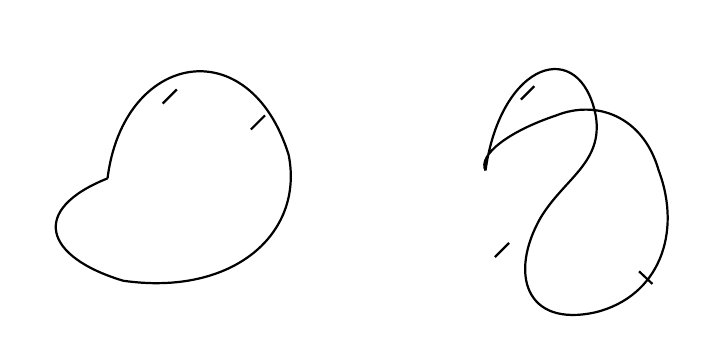
\begin{tikzpicture}[scale=1.0]
\draw[line width=0.8pt] (0,0)
  .. controls (0.2,1.6) and (1.8,1.9) .. (2.3,0.3)
  .. controls (2.5,-0.7) and (1.6,-1.5) .. (0.2,-1.3)
  .. controls (-0.8,-1.0) and (-1.0,-0.4) .. (0,0);
\draw[line width=0.8pt] (0.70,0.95) -- (0.88,1.13);
\draw[line width=0.8pt] (1.82,0.62) -- (2.00,0.80);

\draw[line width=0.8pt] (4.8,0.1)
  .. controls (5.0,1.5) and (6.0,1.8) .. (6.2,0.8)
  .. controls (6.3,0.2) and (5.8,0.0) .. (5.5,-0.5)
  .. controls (5.1,-1.2) and (5.3,-1.9) .. (6.2,-1.7)
  .. controls (7.0,-1.5) and (7.3,-0.7) .. (7.0,0.1)
  .. controls (6.8,0.8) and (6.2,1.0) .. (5.7,0.8)
  .. controls (5.1,0.6) and (4.7,0.3) .. (4.8,0.1);
\draw[line width=0.8pt] (5.25,1.00) -- (5.42,1.17);
\draw[line width=0.8pt] (5.10,-0.82) -- (4.92,-1.00);
\draw[line width=0.8pt] (6.75,-1.18) -- (6.92,-1.34);
\end{tikzpicture}
\caption{圆与变形回路的清晰重构。周长相等意味着内在的一维几何相同。}
\label{fig:c04-intrinsic-redraw}
\end{figure}

\begin{classroomqa}
\audiencequestion{有限线段会是同一种一维空间吗？}
\lecturerresponse{不会。线段有两个端点，而闭合回路没有端点。这一拓扑区别是内在的，不能通过在更大空间中弯曲其中任何一个对象来消除。一旦拓扑固定，线段由其长度表征，闭合回路则由其周长表征。 \lecturetimestamp{00:26:00--00:26:39}}
\end{classroomqa}

\subsection{为什么嵌入有用但并非必需}

我们通过把一维圆放入二维、把二维球面放入三维来将其可视化。这一模式诱使我们要求在讨论三维球面之前必须有一个第四欧几里得维度。这种要求反映的是人类的可视化能力，而不是数学上的必然性。我们的视觉机制演化出来是为了在三维中导航；坐标和度规使我们能够超越这一限制进行推理，而无需构造一个字面意义上的外部视角。

\begin{classroomqa}
\audiencequestion{额外的空间维度可能存在但小到看不见吗？}
\lecturerresponse{是的。几何并不要求所有维度都具有相同的可观测尺度。一个紧致维度可能远小于日常经验所探测的尺度。然而，眼下这一点更简单：无论额外维度在物理上是否存在，定义我们三维空间的内在度规都不需要一个嵌入维度。 \lecturetimestamp{00:29:55--00:30:12}}
\end{classroomqa}

\begin{classroomqa}
\audiencequestion{一个被限制在弯曲线上的居民如何知道这条线是否弯曲？}
\lecturerresponse{仅凭内在测量，它无法知道。想象光和物质被限制在一根光纤中。在不拉伸光纤的情况下弯曲它，会改变嵌入，但不会改变沿光纤测得的距离或信号传播时间。只有逃逸到周围空间中的信号才能揭示外部弯曲。 \lecturetimestamp{00:30:15--00:31:14}}
\end{classroomqa}

这个思想实验可以操作化。一个被限制在光纤中的生物可以发射一个信号，例如一个能量足够高的光子，只有当该信号逃逸出光纤并随后通过一维度规中不可用的路径返回时，它才能发现一个外部方向。本着同样的精神，普通空间具有三个大维度这一陈述归根结底是实验性的，而不是从人类心智能够想象什么推导出来的。

\begin{classroomqa}
\audiencequestion{如果每一个一维空间都是局部平坦的，那么每一个二维空间也必须局部平坦吗？}
\lecturerresponse{不。一张卷成圆柱面的薄片保持内在平坦：它可以在不被拉伸的情况下展开。一个半球面无法在不拉伸或撕裂的情况下展平到平面上，因此它具有内在曲率。每一块足够小的区域看起来都近似欧几里得，但可测量的偏差会在有限尺度上出现。圆柱面与球面之间的对比，正是外在弯曲与内在曲率之间的对比。 \lecturetimestamp{00:31:14--00:35:00}}
\end{classroomqa}

\begin{classroomqa}
\audiencequestion{内在曲率是否必然意味着存在引力场？}
\lecturerresponse{在广义相对论中，时空曲率是潮汐引力的不变量表现。因此，宇宙学空间曲率 \(k/a^2\) 是引力几何的一部分，而不仅仅是想象的外部空间中的弯曲。物质通过爱因斯坦方程影响曲率，但不应把这一陈述强化为“曲率只存在于物质所在之处”：真空时空可以携带外尔曲率，例如在恒星外部或引力波中。 \lecturetimestamp{00:35:01--00:35:51}}
\end{classroomqa}

现在我们施加大尺度理想化。对恒星、星系、星系团和局部不规则性取平均，就像在把地球描述为球形时忽略山脉一样。由此得到的空间几何被假定为均匀且各向同性的。在这些假设下，存在三种常曲率可能性：平坦、球面和双曲。

\section{FRW假设与三种曲率情形}

对称性假设将几何结构压缩为一个随时间变化的尺度因子和一个离散的曲率符号。在共动坐标中，Friedmann-Robertson-Walker 拟设是
\begin{equation}
ds^2=-dt^2+a(t)^2\,d\Sigma_k^2,
\qquad
k\in\{-1,0,+1\}.
\label{eq:c04-frw}
\end{equation}
时间坐标是共动观测者的固有时。均匀性允许 \(a\) 依赖于时间而不依赖于位置，而各向同性则禁止存在一个优先的空间方向。

\begin{figure}[htbp]
\centering
\includegraphics[width=0.74\textwidth]{lecture_04_figure_02.png}
\caption{三个常曲率空间度规被归在共同的尺度因子之下。该画面是后来拍摄的，当时黑板上已经积累了其他内容，但它保留了 00：40：23--00：42：42 的度规讨论。}
\label{fig:c04-frw-board}
\lectureframe{00:45:48.386}
\end{figure}

使用径向坐标 \(r\) 和单位二维球面度规 \(d\Omega_2^2\)，三个归一化空间度规为
\begin{align}
d\Sigma_0^2 &= dr^2+r^2d\Omega_2^2,
&& k=0,
\label{eq:c04-flat-space}\\
d\Sigma_{+1}^2 &= dr^2+\sin^2 r\,d\Omega_2^2,
&& k=+1,
\label{eq:c04-spherical-space}\\
d\Sigma_{-1}^2 &= dr^2+\sinh^2 r\,d\Omega_2^2,
&& k=-1.
\label{eq:c04-hyperbolic-space}
\end{align}
因此，在固定时刻，空间是平坦的、正曲率的或负曲率的。乘以 \(a(t)^2\) 会以相同的因子改变每一个空间距离，同时保持归一化形状不变。

取两个具有固定共动间距 \(\Delta\chi\) 的星系。它们的物理距离为
\begin{equation}
D(t)=a(t)\Delta\chi.
\end{equation}
求导并消去 \(\Delta\chi\) 得到
\begin{equation}
\dot D=\dot a\,\Delta\chi
      =\frac{\dot a}{a}D
      =H(t)D,
\qquad
H(t)\equiv\frac{\dot a}{a}.
\label{eq:c04-hubble-law}
\end{equation}
因此，Hubble 定律从运动学上由均匀标度变换得出。Hubble 参数可以随时间变化，但在任何固定的宇宙时刻，它在各处都相同。

\section{从 Einstein 方程到 Friedmann 方程}

度规告诉我们距离如何测量，但没有告诉我们 \(a(t)\) 如何演化。弯曲时空需要 Einstein 方程。计算每一个 Christoffel 符号和曲率分量会掩盖物理论证，因此我们使用由对称性强制给出的形式，并分离出它的时间-时间分量。

在 \(c=1\) 的单位制下，并暂时略去宇宙学常数，完整的张量方程为
\begin{equation}
G_{\mu\nu}
\equiv
R_{\mu\nu}-\frac12 g_{\mu\nu}R
=8\pi G\,T_{\mu\nu}.
\label{eq:c04-einstein}
\end{equation}
几何量占据左边；能量密度、动量密度、压强和应力占据右边。因子 \(1/3\) 不属于完整张量方程。它只有在时间-时间分量被化为 Friedmann 形式之后才出现。

\begin{figure}[htbp]
\centering
\includegraphics[width=0.78\textwidth]{lecture_04_figure_03.png}
\caption{Einstein 方程的一个中间黑板状态。几何的左侧可见，而物质张量尚不可辨认，且所显示的归一化不完整。方程~\eqref{eq:c04-einstein}记录了推导中使用的标准完整张量方程。}
\label{fig:c04-einstein-board}
\lectureframe{00:48:19.394}
\end{figure}

对于在共动坐标中静止的均匀流体，
\begin{equation}
T_{00}=\rho.
\label{eq:c04-energy-density}
\end{equation}
时间-时间 Einstein 张量具有一个有用的结构性质。它的二阶导数相消，留下一个关于一阶时间导数的二次项和一个来自空间曲率的项：
\begin{equation}
G_{00}=3\left[
\left(\frac{\dot a}{a}\right)^2+\frac{k}{a^2}
\right].
\label{eq:c04-g00}
\end{equation}
将方程~\eqref{eq:c04-energy-density}和\eqref{eq:c04-g00}代入方程~\eqref{eq:c04-einstein}，得到第一个 Friedmann 方程，
\begin{equation}
\boxed{
\left(\frac{\dot a}{a}\right)^2+\frac{k}{a^2}
=\frac{8\pi G}{3}\rho
}.
\label{eq:c04-friedmann}
\end{equation}
等价地，
\begin{equation}
H^2=\frac{8\pi G}{3}\rho-\frac{k}{a^2}.
\label{eq:c04-friedmann-energy}
\end{equation}
方程~\eqref{eq:c04-friedmann-energy}的形式与早先 Newton 论证中得到的形式完全一致。在那里，积分常数被解释为一团物质的总机械能或逃逸条件。广义相对论将内禀空间曲率放在同一个数学位置上。这种一致并非偶然：在足够小的区域内，曲率效应变得可以忽略，相对论宇宙学必须重现局部 Newton 行为。相对论还澄清了 \(\rho\) 意味着总能量密度，因此相对论性粒子和光子也会产生引力，尽管非相对论性的质量密度论证会漏掉它们。

\begin{classroomqa}
\audiencequestion{为什么度规中没有混合空间和时间的项？}
\lecturerresponse{混合项会表现得像相对于共动观测者的一个优先空间矢量或流。严格的均匀性和各向同性不留下任何这样的方向。因此，在适应宇宙物质的坐标中，移位函数消失，度规取方程~\eqref{eq:c04-frw}中的块对角形式。如果所假设的对称性得以保持，这就不是额外的动力学猜测，而是它们的几何推论。 \lecturetimestamp{00:58:27--00:59:08}}
\end{classroomqa}

\begin{classroomqa}
\audiencequestion{为什么时间-时间分量就足够了，二阶导数又到哪里去了？}
\lecturerresponse{均匀且各向同性的拟设只包含一个未知函数 \(a(t)\)。混合分量化为恒等式，而空间分量与时间-时间方程及应力-能量守恒相关。人们可以将它们合并为一个包含 \(\ddot a\) 的加速度方程，但时间-时间爱因斯坦张量是特殊的：它的二阶导数项相消，留下了一阶能量方程~\eqref{eq:c04-friedmann}。一个非平凡方程加上物质演化定律，就足以确定这唯一的几何自由度。\lecturetimestamp{00:59:09--01:00:56}}
\end{classroomqa}

\section{宇宙的内容物如何稀释}

在 \(\rho\) 作为 \(a\) 的函数已知之前，弗里德曼方程并不闭合。几何已经提供了一个方程；宇宙中的物质必须提供第二个关系。

对于非相对论性物质，共动体积内的粒子数是固定的，而物理体积按 \(a^3\) 增长。忽略粒子的小动能，
\begin{equation}
\rho_{\mathrm m}(a)=\frac{\rho_{\mathrm m,0}}{a^3}.
\label{eq:c04-matter-scaling}
\end{equation}
这里归一化 \(a=1\) 可以在任何方便的参考时期指定；只有标度因子的比值才具有直接意义。

\begin{classroomqa}
\audiencequestion{如果平坦宇宙是无限的，那么 \(a\) 向大爆炸收缩意味着什么？}
\lecturerresponse{对于 \(a\) 的每一个非零值，无限平坦空间仍然是无限的；所有有限的共动间隔都乘以同一个收缩因子。在平坦情形下，\(a\) 的绝对归一化是任意的，因此只有 \(a(t_2)/a(t_1)\) 具有不变意义。对于闭合的球形宇宙，\(a\) 自然是其曲率半径；对于双曲宇宙，它设定了曲率半径。极限 \(a\to0\) 标志着宇宙学奇点，而不是一个位于外部空间中的普通有限球。\lecturetimestamp{01:05:06--01:05:53}}
\end{classroomqa}

辐射以两种方式损失能量。其数密度按体积的倒数下降，而每个光子的波长按 \(a\) 成比例拉伸，使其能量再减少一个 \(a^{-1}\) 因子。因此
\begin{equation}
\rho_{\mathrm r}(a)=\frac{\rho_{\mathrm r,0}}{a^4}.
\label{eq:c04-radiation-scaling}
\end{equation}
因为 \(a^{-4}\) 向过去增长得比 \(a^{-3}\) 更快，所以即使物质在晚得多的时候占主导，辐射在足够早的时期也会占主导。

如果物质和辐射是仅有的组分，那么 \(k\) 的符号将强烈地预示未来：\(k=+1\) 允许再坍缩，\(k=0\) 是永远膨胀但减速的临界情形，而 \(k=-1\) 永远膨胀且曲率最终变得重要。暗能量打破了这种简单的联系。闭合宇宙可以永远膨胀，而空间平坦性本身并不能决定最终命运。

\section{状态方程与连续性定律}

与其为每种物质记住一条单独的稀释规则，不如用状态方程来表征物质。该方案有两部分。首先，对于给定的压强与能量密度之间的关系，推导出 \(\rho(a)\)。然后，从物质、辐射或真空的微观物理确定该关系。对于本讲而言，第一部分就足够了。

压强是动量通量。撞击盒子壁的分子反转其动量并推压壁；更快的粒子传递更多动量并产生更大的压强。因此，一旦指定了物质种类，能量密度和压强就不能独立选择。对于一个简单的宇宙学组分，我们写
\begin{equation}
P=w\rho,
\label{eq:c04-equation-state}
\end{equation}
其中在 \(c=1\) 的单位制下，\(w\) 是无量纲的。冷物质压强可忽略，因此 \(w=0\)。辐射有 \(w=1/3\)，其中因子 \(1/3\) 反映了对三个空间方向的平均。

\begin{figure}[htbp]
\centering
\includegraphics[width=0.82\textwidth]{lecture_04_figure_06.png}
\caption{黑板上收集了物质和辐射的标度关系，并将状态方程写为 \(P=W\rho\)。我们使用约定的小写 \(w\)。}
\label{fig:c04-equation-state-board}
\lectureframe{01:15:08.166}
\end{figure}

\subsection{共动盒子中的热力学}

取一个共动盒子，其物理体积为\(V\)，能量密度为\(\rho\)，总能量为
\begin{equation}
E=\rho V.
\end{equation}
第一定律为
\begin{equation}
dE=T\,dS-P\,dV.
\end{equation}
宇宙学膨胀被当作绝热过程处理，因此对于该共动盒子有\(dS=0\)，并且
\begin{equation}
dE=-P\,dV.
\label{eq:c04-adiabatic-first-law}
\end{equation}
负号表示膨胀的系统对外做功并损失内能。对\(E=\rho V\)独立求导得到
\begin{equation}
dE=\rho\,dV+V\,d\rho.
\end{equation}
令两式相等，
\begin{align}
\rho\,dV+V\,d\rho&=-P\,dV,\\
V\,d\rho&=-(\rho+P)\,dV.
\label{eq:c04-volume-continuity}
\end{align}
以\(P=w\rho\)代入，
\begin{equation}
\frac{d\rho}{\rho}=-(1+w)\frac{dV}{V}.
\end{equation}
积分给出
\begin{equation}
\rho\propto V^{-(1+w)}.
\end{equation}
由于共动体积按\(V\propto a^3\)标度，
\begin{equation}
\boxed{\rho(a)\propto a^{-3(1+w)}}.
\label{eq:c04-density-scaling}
\end{equation}
写成微分形式，同一陈述即为局域能量守恒方程
\begin{equation}
\dot\rho+3H(\rho+P)=0.
\label{eq:c04-continuity}
\end{equation}
即使变化的宇宙学几何未必允许存在全局守恒的总能量，这一局域守恒定律仍然精确成立。

两个熟悉的情形随即得出：
\begin{align}
w=0
&\quad\Longrightarrow\quad
\rho_{\mathrm m}\propto a^{-3},\\
w=\frac13
&\quad\Longrightarrow\quad
\rho_{\mathrm r}\propto a^{-4}.
\end{align}
辐射多出的那个逆幂次是宇宙学红移的热力学表达。

\begin{classroomqa}
\audiencequestion{今天宇宙中还剩下什么辐射？}
\lecturerresponse{课堂讨论主要指向宇宙微波背景，即来自炽热早期宇宙的遗留光子浴。辐射目前只占宇宙总能量密度的一小部分，但其\(a^{-4}\)标度意味着，当方程往回推得足够远时，它会超过物质。当前各成分的精确比例是观测输入，这一标度论证并不需要它们。\lecturetimestamp{01:26:53--01:28:34}}
\end{classroomqa}

\section{真空能与曲率决定命运规则的失效}

暗能量引入状态方程
\begin{equation}
P=-\rho,
\qquad
w=-1.
\label{eq:c04-vacuum-eos}
\end{equation}
负压就是张力：盒内的东西不是向外推盒壁，而是向内拉盒壁。拉伸的弹簧是常见的具有张力的物体，不过这只是一种类比，并不是真空能的微观模型。

\begin{classroomqa}
\audiencequestion{负压与绝对零度有关吗？}
\lecturerresponse{并不存在任何简单的一般性关联。把普通材料冷却到零温，本身并不会产生宇宙学状态方程\(P=-\rho\)。这一对照之所以有用，是因为它把热压强与真空应力区分开来：真空能由洛伦兹不变的应力-能量张量刻画，其空间分量表现为负压。它的微观起源则是另一个问题。\lecturetimestamp{01:31:01--01:31:46}}
\end{classroomqa}

将\(w=-1\)代入方程~\eqref{eq:c04-density-scaling}得到
\begin{equation}
\rho_\Lambda\propto a^0=\text{constant}.
\label{eq:c04-vacuum-density}
\end{equation}
当共动区域膨胀时，其体积与总真空能一同增大，从而使单位体积的能量保持不变。方程~\eqref{eq:c04-adiabatic-first-law}中的功项解释了这一行为，因为\(P\)为负。一旦存在这样的成分，正的空间曲率就不再保证再坍缩。

\begin{classroomqa}
\audiencequestion{暗物质、黑洞以及其他致密天体如何纳入？}
\lecturerresponse{在远大于它们彼此间距的尺度上，任何随机速度很小的非相对论性成分都属于无压物质密度。这包括普通物质、冷暗物质，以及诸如黑洞之类的致密天体族群。它们的局部结构很复杂，但粗粒化之后，其平均宇宙学状态方程近似为\(w=0\)。\lecturetimestamp{01:33:34--01:34:10}}
\end{classroomqa}

\begin{classroomqa}
\audiencequestion{相对论性方程会重现此前得到的物质主导和辐射主导解吗？}
\lecturerresponse{会。对于\(k=0\)，将\(\rho_{\mathrm m}\propto a^{-3}\)代入弗里德曼方程得到\(\dot a^2\propto a^{-1}\)，因而\(a(t)\propto t^{2/3}\)。代入\(\rho_{\mathrm r}\propto a^{-4}\)得到\(\dot a^2\propto a^{-2}\)以及\(a(t)\propto t^{1/2}\)。广义相对论改变了诠释并扩大了可能的源，但它保留了这些解。\lecturetimestamp{01:34:14--01:35:12}}
\end{classroomqa}

\begin{classroomqa}
\audiencequestion{在牛顿图像中，暗能量会类似于什么样的力？}
\lecturerresponse{正的宇宙学常数产生与间距成正比的排斥性相对加速度，
\[
\ddot D=\frac{\Lambda}{3}D
\]
在\(c=1\)的单位制下。负的宇宙学常数则改变符号，表现为吸引。由于正\(\Lambda\)效应随距离增大，它最终可以主导物质和曲率；即便是一个闭合的\(k=+1\)宇宙，此后也能继续膨胀。这种牛顿形式只是相对论动力学的一个有用影子。\lecturetimestamp{01:35:13--01:36:55}}
\end{classroomqa}

\section{需要带走的内容}

宇宙学原理是一个平均化的几何断言：在局部结构被抹平之后，每一点和每一方向都等价。它把空间度规限制为三种常曲率情形，并把所有时间依赖打包进\(a(t)\)：
\begin{equation}
ds^2=-dt^2+a(t)^2d\Sigma_k^2.
\end{equation}
于是共动间距满足\(\dot D=HD\)，而束缚系统则不必加入这一流动。

爱因斯坦的时间-时间方程将这一试探解转化为动力学：
\begin{equation}
H^2+\frac{k}{a^2}=\frac{8\pi G}{3}\rho.
\end{equation}
它与牛顿能量方程的相似性是真实的，但广义相对论将积分项等同于内禀空间曲率，并允许每一种形式的能量都作出贡献。

剩下的输入是热力学方面的。对于一个绝热膨胀的组分，若\(P=w\rho\)，则
\begin{equation}
\dot\rho+3H(\rho+P)=0,
\qquad
\rho\propto a^{-3(1+w)}.
\end{equation}
物质、辐射和真空能分别对应于
\begin{equation}
w=0,\qquad w=\frac13,\qquad w=-1.
\end{equation}
它们不同的稀释速率决定了在每个时期哪一种组分主导膨胀。接下来的任务是理解这些状态方程背后的物理，以及真空能所产生的加速。